\PassOptionsToPackage{unicode=true}{hyperref} % options for packages loaded elsewhere
\PassOptionsToPackage{hyphens}{url}
%
\documentclass[]{article}
\usepackage{mypackages}
\usepackage{lmodern}
\usepackage{amssymb,amsmath}
\usepackage{ifxetex,ifluatex}
\usepackage{lscape}
\usepackage{graphicx}
\usepackage{float}
%    \usepackage{lscape}
\usepackage{rotating}
\usepackage{fixltx2e} % provides \textsubscript
\ifnum 0\ifxetex 1\fi\ifluatex 1\fi=0 % if pdftex
  \usepackage[T1]{fontenc}
  \usepackage[utf8]{inputenc}
  \usepackage{textcomp} % provides euro and other symbols
\else % if luatex or xelatex
  \usepackage{unicode-math}
  \defaultfontfeatures{Ligatures=TeX,Scale=MatchLowercase}
\fi
% use upquote if available, for straight quotes in verbatim environments
\IfFileExists{upquote.sty}{\usepackage{upquote}}{}
% use microtype if available
\IfFileExists{microtype.sty}{%
\usepackage[]{microtype}
\UseMicrotypeSet[protrusion]{basicmath} % disable protrusion for tt fonts
}{}
\IfFileExists{parskip.sty}{%
\usepackage{parskip}
}{% else
\setlength{\parindent}{0pt}
\setlength{\parskip}{6pt plus 2pt minus 1pt}
}
\usepackage{hyperref}
\hypersetup{
            pdftitle={arc42 Template},
            pdfborder={0 0 0},
            breaklinks=true}
\urlstyle{same}  % don't use monospace font for urls
\usepackage{longtable,booktabs}
% Fix footnotes in tables (requires footnote package)
\IfFileExists{footnote.sty}{\usepackage{footnote}\makesavenoteenv{longtable}}{}
\usepackage{graphicx,grffile}
\makeatletter
\def\maxwidth{\ifdim\Gin@nat@width>\linewidth\linewidth\else\Gin@nat@width\fi}
\def\maxheight{\ifdim\Gin@nat@height>\textheight\textheight\else\Gin@nat@height\fi}
\makeatother
% Scale images if necessary, so that they will not overflow the page
% margins by default, and it is still possible to overwrite the defaults
% using explicit options in \includegraphics[width, height, ...]{}
\setkeys{Gin}{width=\maxwidth,height=\maxheight,keepaspectratio}
\setlength{\emergencystretch}{3em}  % prevent overfull lines
\providecommand{\tightlist}{%
  \setlength{\itemsep}{0pt}\setlength{\parskip}{0pt}}
\setcounter{secnumdepth}{0}
% Redefines (sub)paragraphs to behave more like sections
\ifx\paragraph\undefined\else
\let\oldparagraph\paragraph
\renewcommand{\paragraph}[1]{\oldparagraph{#1}\mbox{}}
\fi
\ifx\subparagraph\undefined\else
\let\oldsubparagraph\subparagraph
\renewcommand{\subparagraph}[1]{\oldsubparagraph{#1}\mbox{}}
\fi

% set default figure placement to htbp
\makeatletter
\def\fps@figure{htbp}
\makeatother


%\title{
\includegraphics{images/arc42-logo.png} Template}
%\date{2019-01-04}
%###############################################################################
% Grössenangaben zum Dokument etc.\cite{Michaelis}

% vertikal
%\setlength{\voffset}{-0.5cm}
%\setlength{\textheight}{23cm}
%\setlength{\topmargin}{0cm}
%\setlength{\headheight}{6mm}
%\setlength{\headsep}{1cm}
%\setlength{\topskip}{0cm}
%\setlength{\footskip}{1cm}
%
%% horizontal
%\setlength{\hoffset}{-0.4cm}
%\setlength{\textwidth}{15.5cm}
%\setlength{\oddsidemargin}{0.8cm}
%\setlength{\evensidemargin}{0.8cm}
%
%\setlength{\parindent}{0cm}        % kein Einzug bei Paragrafenbeginn


%###############################################################################
% Autor und Abgabedatum ändern
\def\autor{Nikolas Rist, Kai Bepperling}
\def\datum{20.~September 2019}
\begin{document}
% Titelseite

%\sloppy
%\pagestyle{headings}
%\pagenumbering{roman}

% Basierend auf der Fachschaftsvorlage
\begin{titlepage}
	\textbf{
		\begin{tabular}[t]{>{\vspace*{0pt}}p{0.45\textwidth}c>{\vspace*{0pt}}p{0.45\textwidth}}
			{
				\begin{tabular}{ll}
					\begin{tabular}{l}
						\raisebox{1.5\height}{
\includegraphics[width=0.13\textwidth]{images/fhlogo.png}} 
					\end{tabular}
					&
					\begin{tabular}{l}
						{\small{\sffamily Hochschule}}\\
						{\small{\sffamily Bonn-Rhein-Sieg}}\\
						{\footnotesize{\itshape University of Applied Sciences}}\\
						\\
						{\small{\sffamily Fachbereich Informatik}}\\
						{\footnotesize{\itshape Computer Science Department}}\\
					\end{tabular}
				\end{tabular}
			}
			&
			\hspace*{0.1\textwidth}
		\end{tabular}
	} %\textbf
	
	
	\renewcommand{\baselinestretch}{1.4}\normalsize
	
	\vspace{3cm}
	\begin{center}
		
		% einen Typ auswählen
		\begin{Huge}\textbf{Semesterprojekt}\end{Huge}\\
		\vspace{0.8cm}
		% einen Studiengang auswählen
		\begin{Large}\textbf{Serviceorientierte Architekturen im Masterstudiengang Informatik}\end{Large}\\
		
		\vspace{2.2cm}
		\renewcommand{\baselinestretch}{1.2}\normalsize
		\begin{huge}
			\textbf{HighPerformance}
		\end{huge}
		\renewcommand{\baselinestretch}{1.5}\normalsize
		\\
		\vspace{0.8cm}
		\begin{Large}
			\textbf{}
		\end{Large}
		
		\vspace{0.7cm}
		\begin{Large}\textbf{von \autor\ \\}
		\end{Large}
	\end{center}
	
	\vspace{2cm}
	
	\begin{large}
		\textbf{
			\begin{tabular}{ll}
				Erstprüfer:  & Prof. Dr. Sascha Alda\\
%				Zweitprüfer:  & - \\
				Eingereicht am: & \datum\ \\
			\end{tabular}
		}
	\end{large}
\end{titlepage}

\tableofcontents
\cleardoublepage
%\pagenumbering{arabic}

\hypertarget{section-introduction-and-goals}{%
\section{Einführung und Ziele}\label{section-introduction-and-goals}}
Ziel des Projekts ist die Optimierung der Performanceevaluierung der Mitarbeiter der \emph{SmartHoover Ltd.} Im Vorraus wurden Interviews mit den Stakeholdern geführt, um das Projekt konkret definieren zu können. 

\hypertarget{_aufgabenstellung}{%
\subsection{Aufgabenstellung}\label{_aufgabenstellung}}

Der bisherige Prozess erfodert viele manuelle Schritte und findet zum Großteil auf Papier statt. Die Informationen sind allerdings in den Systemen OpenCRX und OrangeHRM bereits vorhanden und sollen auch zukünftig genutzt werden. 
Die verschiedenen Stakeholder, welche im Abschnitt \ref{_stakeholder} beschrieben werden, haben in einem Interview einige Anforderungen an das neue System gestellt.
\subsubsection{CEO}
\begin{itemize}
\item Die berechneten Boni müssen manuell freigegebn werden.
\item Änderung der brechneten Boni muss vor Freigabe möglich sein.
\item Vereinfachung des gesamten Prozesses durch weniger manuelle Schritte.
\end{itemize}

\subsubsection{Senior HR Consultant}
\begin{itemize}
	\item Der Prozess muss beschleunigt werden.
	\item Weniger manuelle Interaktionen mit den Systemen OrangeHRM, OpenCRX und dem Datenbanktool.
	\item Weniger Papierarbeit.
\end{itemize}

\subsubsection{IT-Admin}
\begin{itemize}
 \item Loslösung aus dem Prozess.
\end{itemize}

\subsection{Szenarien}
In diesem Abschnitt werden zwei mögliche Nutzungszenarien dargestellt.
\begin{figure}
	\centering
	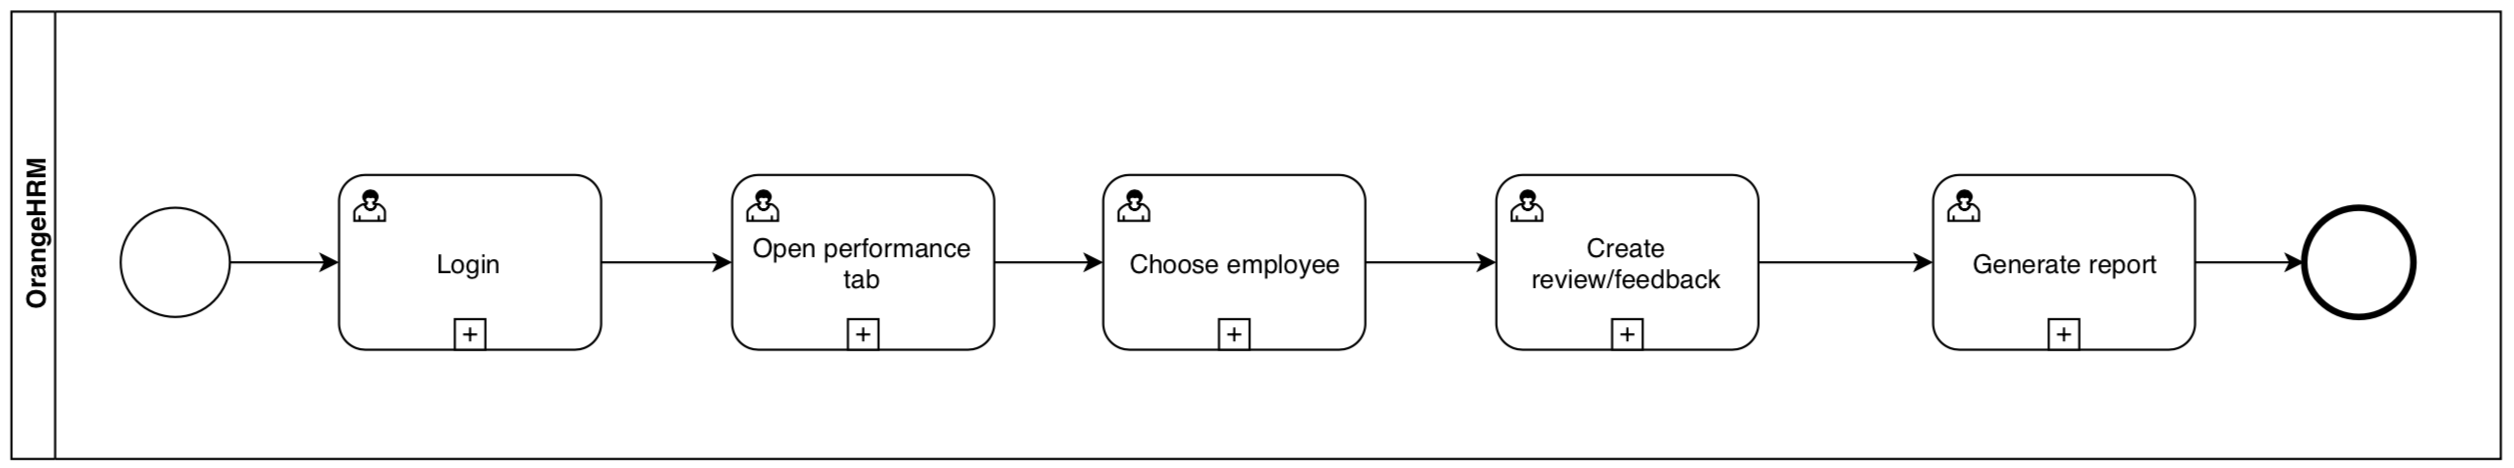
\includegraphics[width=1.0\linewidth]{images/szenario1}
	\caption{Manuelle Berechnung der Boni}
	\label{fig:szenario1}
\end{figure}

\begin{figure}
	\centering
	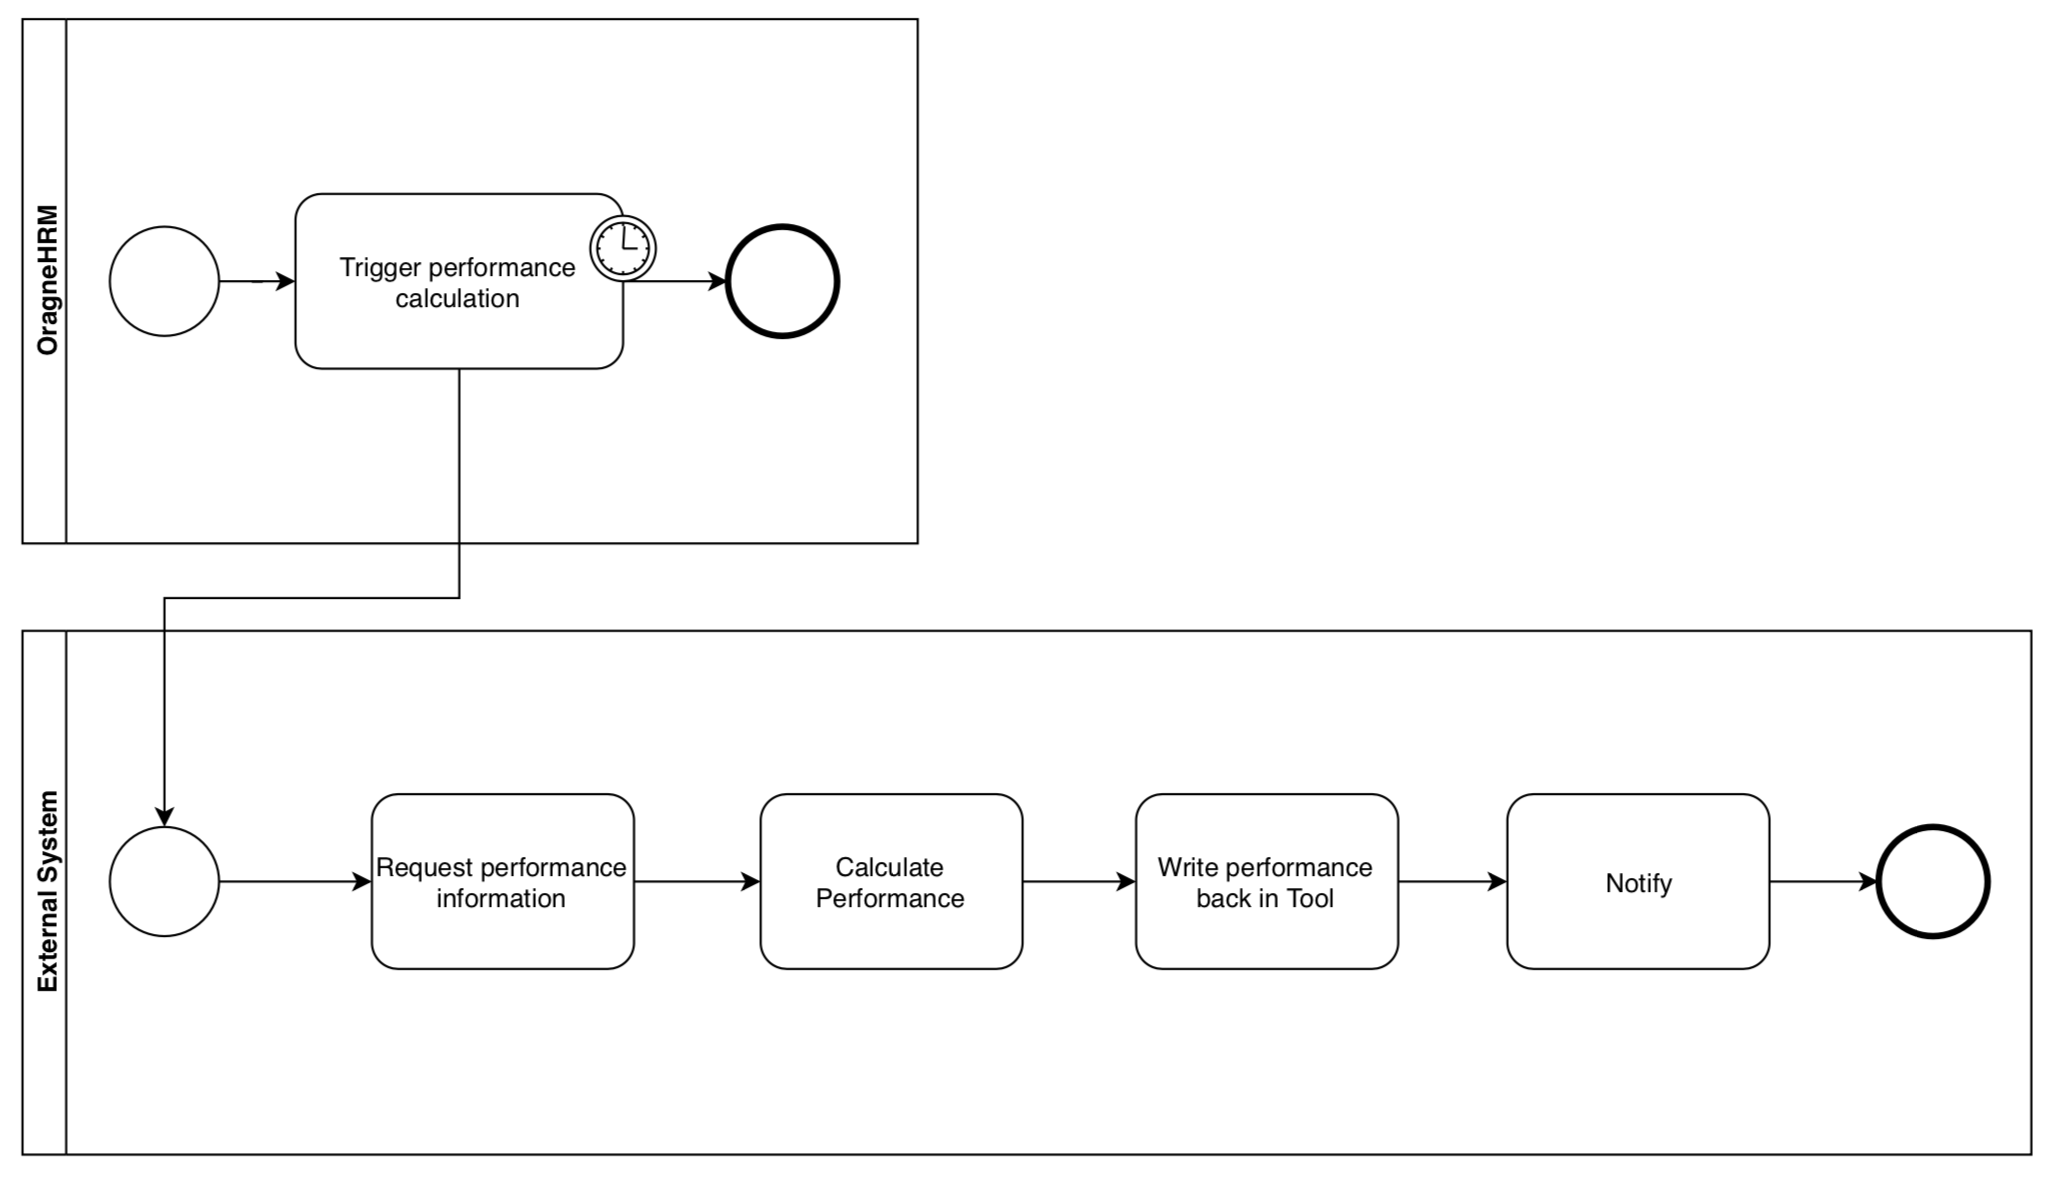
\includegraphics[width=1.0\linewidth]{images/szenario2}
	\caption{Vollautomatisierte Berechnung der Boni}
	\label{fig:szenario2}
\end{figure}


\hypertarget{_qualit_tsziele}{%
\subsection{Qualitätsziele}\label{_qualit_tsziele}}

\begin{enumerate}
\item Prozessbeschleunigung
\item Weniger manuelle Schritte
\item Weniger Prozessteilnehmer
\end{enumerate}


\hypertarget{_stakeholder}{%
\subsection{Stakeholder}\label{_stakeholder}}

\begin{longtable}[]{@{}lll@{}}
\toprule
\begin{minipage}[b]{0.23\columnwidth}\raggedright
Rolle\strut
\end{minipage} & \begin{minipage}[b]{0.23\columnwidth}\raggedright
Kontakt\strut
\end{minipage} & \begin{minipage}[b]{0.46\columnwidth}\raggedright
Erwartungshaltung\strut
\end{minipage}\tabularnewline
\midrule
\endhead
\begin{minipage}[t]{0.23\columnwidth}\raggedright
	\emph{CEO}\strut
\end{minipage} & \begin{minipage}[t]{0.23\columnwidth}\raggedright
\emph{Dr. Michael Moore}\strut
\end{minipage} & \begin{minipage}[t]{0.46\columnwidth}\raggedright
\emph{Keine Vollautomatisierung, Segnet alle Boni manuell ab}\strut
\end{minipage}\tabularnewline
\begin{minipage}[t]{0.23\columnwidth}\raggedright
\emph{HR Senior Consultant}\strut
\end{minipage} & \begin{minipage}[t]{0.23\columnwidth}\raggedright
\emph{Chantal Banks}\strut
\end{minipage} & \begin{minipage}[t]{0.46\columnwidth}\raggedright
\emph{Weniger manuelle Schritte, Keine Papierarbeit mehr}\strut
\end{minipage}\tabularnewline
\begin{minipage}[t]{0.23\columnwidth}\raggedright
	\emph{IT-Admin}\strut
\end{minipage} & \begin{minipage}[t]{0.23\columnwidth}\raggedright
	\emph{Tom Foster}\strut
\end{minipage} & \begin{minipage}[t]{0.46\columnwidth}\raggedright
	\emph{Keine Berührungspunkte mit dem gesamten Prozess}\strut
\end{minipage}\tabularnewline
\bottomrule
\end{longtable}


\hypertarget{section-architecture-constraints}{%
\section{Randbedingungen}\label{section-architecture-constraints}}

Beschreibung der zu nutzenden externen Systemen

\textbf{Was ist die prinzipielle Aufgabe der Anwendung OpenCRX? }
\begin{itemize}
\item CRM System
\item Account management
\item Product and Price Management
\item Sales Pipeline
\item Issue tracking
\item Groupware
\item mail, contact and calendar management
\end{itemize}

\textbf{Was ist die prinzipielle Aufgabe der Anwendung OrangeHRM? }
\begin{itemize}
	\item Resource Management
	\item performance Management
	\item  Administration and Personal Information Management
	\item  Recruitment etc.
	\item  Employee Self Service (Time Tracking)
\end{itemize}

\textbf{Welche grundlegenden Funktionen besitzen diese Anwendungen?}
OrangeHRM bietet Funktionalitäten zum Verwalten des Personals und alles was dazu gehört:
\begin{itemize}
	\item Mitarbeiterverwaltung inkl. Mitarbeiter Self Service
	\item Dashboards
	\item Mitarbeiter Training
	\item Reiseplanung
	\item Dokumentenmanager
	\item OpenCRX bietet Funktionalitäten zur Verwaltung von Kunden
	\item Kundensupport
	\item Customer Success
	\item Marketing
	\item Analytics
	\item Sales Management
\end{itemize}

\textbf{Welche Geschäftsobjekte werden in OpenCRX bzw. OrangeHRM verwaltet?}
\begin{itemize}
	\item Kunden
	\item Mitarbeiter
\end{itemize}
\textbf{Welche Art Schnittstellen bieten OpenCRX bzw. OrangeHRM an?}
	\begin{itemize}
	\item OpenCRX:
	\begin{itemize}
		\item RESTful API
		\item AirSync ActiveSync
		\item User Interface (WebUI)
	\end{itemize}
	\item OrangeHRM:
		\begin{itemize}
			\item RESTful API
			\item Mobile APP
			\item User Interface (WebUI)
		\end{itemize}
\end{itemize}


\hypertarget{section-system-scope-and-context}{%
\section{Kontextabgrenzung}\label{section-system-scope-and-context}}

\hypertarget{_fachlicher_kontext}{%
\subsection{Fachlicher Kontext}\label{_fachlicher_kontext}}

Der Prozess kann von einem HR Senior über das Userinterface der Camunda Plattform (Tasklist) gestartet werden. Beim Start muss der entsprechende Mitarbeiter in das angebotene Formular-Feld eingetragen werden.

Weiterhin wird dem CEO in Camunda ein entsprechendes Formular mit einer Aufstellung der berechneten Boni zur Verfügung gestellt.
In diesen kann er Korrekturen an den einzelnen Boni vornehmen und entsprechend speichern damit diese im fortlaufenden Prozess berücksichtigt werden.

\hypertarget{_technischer_kontext}{%
\subsection{Technischer Kontext}\label{_technischer_kontext}}

Die Camunda-Engine nutzt die bereitgestellte RESTful-Schnittstelle des Data-Colletors, um entsprechende Informationen über den zu bearbeitenden Salesman auszutauschen.
Hierbei wird das sogenannte ClientInfoDTO ausgetauscht.

\textbf{Data Collector - Objekte}
\begin{verbatim}
data class ClientInfoDTO(
    var salesmanName: String = "",
    var salesInfos: ArrayList<SalesInfoDTO> = ArrayList()
)

data class SalesInfoDTO(
    var productName: String = "",
    var clientName: String = "",
    var clientRanking: Int = 0,
    var quantity: Double = 0.0,
    var bonus: Int = 0
)
\end{verbatim}

Zum kommunizieren mit den externen Systemen, OrangeHRM und OpenCRX, nutzt der Data-Collector eine entsprechende RESTful Schnittstelle.

\textbf{OrangeHRM - Objekte}
\begin{verbatim}
	data class Employee(
    val firstName: String,
    val lastName: String,
    val employeeId: String,
    val jobTitle: String
)

data class Organization(
    val id: String,
    val name: String,
    val email: String?,
    val country: String,
    val numberOfEmployees: String
)
\end{verbatim}

\textbf{OpenCRX - Objekte}
\begin{verbatim}
	data class Account(
    val firstName: String? = "",
    val lastName: String? = "",
    val fullName: String? = "",
    val familyStatus: Int = 0,
    val organization: String? = "",
    val jobTitle: String? = "",
    val gender: Int = 0,
    val preferredSpokenLanguage: Int = 0,
    val accountRating: Int = 0,
    val industry: String? = "",
    val annualIncomeCurrency: Int = 0,
    @JsonProperty("@href") val accountUrl: String? = ""
)
\end{verbatim}

Abbildung \ref{fig:uebung64kontextsicht} zeigt die entsprechenden Kommunikationskanäle via HTTP zwischen den technischen Systemen.

\begin{figure}[H]
	\centering
	\includegraphics[width=1.0\linewidth]{"images/uebung6_4_kontext_sicht"}
	\caption{Kontext des Systems}
	\label{fig:uebung64kontextsicht}
\end{figure}

\hypertarget{section-building-block-view}{%
\section{Bausteinsicht}\label{section-building-block-view}}

\begin{figure}[H]
	\centering
	\includegraphics[width=1.0\linewidth]{"images/uebung6_4_baustein_sicht"}
	\caption{Bausteinsicht}
	\label{fig:uebung64bausteinsicht}
\end{figure}


\hypertarget{section-runtime-view}{\section{Laufzeitsicht}\label{section-runtime-view}}
\begin{figure}[H]
	\centering
	\rotatebox{90}{\includegraphics[width=1.4\linewidth]{"images/laufzeitsicht_high_performance_bpmn"}}
	\caption{Laufzeitsicht}
	\label{fig:laufzeitsichthighperformancebpmn}
\end{figure}


\hypertarget{section-deployment-view}{%
\section{Verteilungssicht}\label{section-deployment-view}}
\begin{figure}[H]
	\centering
	\includegraphics[width=1.0\linewidth]{"images/verteilungssicht"}
	\caption{Verteilungssicht}
	\label{fig:verteilungssicht}
\end{figure}


\hypertarget{section-concepts}{%
\section{Querschnittliche Konzepte}\label{section-concepts}}


Dieser Abschnitt beschreibt übergreifende, prinzipielle Regelungen und
Lösungsansätze, die an mehreren Stellen (=\emph{querschittlich})
relevant sind.

\textbf{Architekturstil}\\
Wir nutzen das Architektur-Muster der Microservices, da wir einen Integrations-Service zwischen den einzelnen Systemen benötigen.
Dieser soll nur durch eine RESTful-API abstrahiert und darüber angesprochen werden.
Diese Abstraktion bietet die Möglichkeit den Service auszutauschen, ohne die Camunda-Platform anpassen zu müssen. 

\textbf{Deployment}\\
Das einfache Austauschen wird begünstigt durch die Entscheidung, den Service als Docker-Container zur Verfügung zu stellen und zu betreiben.
Somit ist er Plattform unabhängig und kann im Bedarfsfalls mehrfach deployed werden.

\textbf{Workflow-Engine}\\
Die Camunda-Platform wurde als Basis für die Workflow-Implementierung genutzt, da sie eine out-of-the-box Nutzeroberfläche zur Verfügung stellt und somit einen guten Überblick für nicht-technische Mitarbeiter ermöglicht.
Weiterhin kann der gesamte Prozess mittels BPMN standardisiert visualisiert werden. Camunda bietet des Weiteren ein Nutzeroberfläche, um den aktuellen Stand des Prozesses detailliert zu betrachten.

\textbf{Data-Collector}\\
Der Data-Collector bildet das Herzstück des Gesamtsystems, da es alle drei genutzten Services OpenCRX, OrangeHRM und Camunda miteinander verbindet.
Dieser Service wurde in der Sprache Kotlin, mit dem Web-Framework Ktor, entwickelt. 
Ktor bietet einen modular aufgebauten Web-Server, mit dem man leichtgewichtige RESTful APIs implementieren kann.
Kotlin und Ktor sind \emph{state-of-the-art} Technologien.
Für eine Weiterentwicklung des Services besteht durch eine solch junge Programmiersprache allerdings kein Risiko, da Kotlin inherent mit Java verwendet werden kann.

\hypertarget{section-design-decisions}{%
\section{Entwurfsentscheidungen}\label{section-design-decisions}}

Zur prototypischen Implementierung wurden verschiedene Sprachen und Technologien verwendet, welche in diesem Abschnitt erläutert werden.

Wie vorgegeben wurde zur modellierung des Workflows das Tool Camunda eingesetzt. Mithilfe von Camunda wurde der gesamte Prozess modeliert und ausgeführt. Das Camunda Cockpit und die Tasklist eignen sich hervorragend zum starten und verwalten der Prozesse. 
Da im verlaufe des Prozesses auch mit Fremdsystemen kommuniziert werden muss, wurde ein Microservice in der Sprache Kotlin entwickelt. Dieser Service übernimmt die Kommunikation mit OrangeHRM und OpenCRX über die dokumentierten RESTful API's.
Um eine konsistene Architektur bereitzustellen bietet der Microservce ebenfalls RESTful-Schnittstellen an, welche aus der JavaDelegate Klasse aus Camunda heraus aufgerufen wird. 
Alle Anwendungen werden in eigenen, weitesgehend isolierten, und orechestriert in Docker Containern bereitgestellt.


\hypertarget{section-technical-risks}{%
\section{Retroperspektive}\label{section-technical-risks}}
\subsection{Skalierung}
In der aktuellen prototypischen Implementierung exisitieren zwei Skalierungsprobleme. Die erste Herausforderung ist das starten des Prozesses. In der aktuellen Implementierung kann die Bonusberechnung nur für einen Mitarbeiter durchgeführt werden. In einer Weiterentwicklung des Tools müsste es erreicht werden, dass der Prozess automatisch alle Salesmen herausfiltert und die Bonusberechnung startet. 
Das zweite Problem bezüglich der Skalierung ist die Anforderung, dass der CEO Michael Moore die berechneten Boni manuell überprüfen und freigeben muss. 
Der implementierte Microservice \emph{data-collector} wurde von Beginn an skalierbar entwickelt, sodass ausschließlich die Anforderung auf Kundenseite angepasst werden muss.

\subsection{Risiken und Herausforderungen}
Im Verlaufe des Projekts haben sich einige Teilbereiche als Herausforderung dargestellt. Der Informationsaustausch zwischen Camunda und dem Microservice bzw. der Entscheidungstabelle war aufgrund unpräziser Dokumentation schwierig. Ebenso war die Erstellung der Camunda Forms nicht offensichtlich dokumentiert, sodass eine weitreichende Recherche durchgeführt werden musste.

Es stellte sich außerdem heraus dass die eingesetzten Fremdsysteme OpenCRX und OrangeHRM komplex modelierte API's anbieten. Bei OrangeHRM sind zwei verschiedene API versionen dokumentiert, wobei nur eine spezielle Version eingesetzt wird, welche allerdings nicht alle Funktionalitäten anbietet. Aus diesem Grund musste für das Zurückschreiben der berechneten Boni ein \emph{custom-field} angelegt werden.
\subsection{Offene Punkte}
In diesem Abschnitt werden die offenen Punkte der prototypischen Implementierung aufgezeigt
\begin{itemize}
	\item Automatische Prozesswiederholung
	\item Automatische Zuweisung des Prozesses an CEO
	\item Berechnung für alle Salesmen
	\item Vollautomatisierung (beschränkt durch Anforderungen des Kunden)
	\item API Clients in eigene Services extrahieren
\end{itemize}

\end{document}
